%% Generic short report include by Mateusz Machalica
%
\documentclass[a4paper]{article}

\usepackage[T1]{fontenc}
% this needs to be loaded before babel-polish
\usepackage{amssymb}
\usepackage{amsmath}
\usepackage{amsthm}
\usepackage[english]{babel}
\usepackage[utf8]{inputenc}
\usepackage[margin=2cm]{geometry}
\usepackage{graphicx}
\usepackage{ifthen}
\usepackage{hyperref}
\usepackage{algorithm}
\usepackage{algpseudocode}
\usepackage{wrapfig}
\usepackage{tikz}
\usepackage{float}
\usepackage{siunitx}
\usepackage{caption}
\usepackage{placeins}

\renewcommand*{\arraystretch}{1.5}

\newcommand{\makeheader}[3]{
  \begin{center}
    \begin{tabular*}{\textwidth}{@{\extracolsep{\fill}}lr}
      #2 & \ifthenelse{\equal{#3}{}}{\today ~r.}{#3} \\[4pt]
      \multicolumn{2}{c}{{\Large #1}} \\[4pt]
      \hline
    \end{tabular*}
    \vspace{4pt}
  \end{center}
}

\sisetup{
  output-decimal-marker = {.},
  separate-uncertainty = true,
  output-open-uncertainty = (,
  output-close-uncertainty = ),
  uncertainty-separator = \pm
}

\newcommand{\floor}[1]{ \lfloor #1 \rfloor }
\newcommand{\ceil}[1]{ \lceil #1 \rceil }
\newcommand{\floorfrac}[2]{ \floor{\frac{#1}{#2}} }
\newcommand{\ceilfrac}[2]{ \ceil{\frac{#1}{#2}} }
\newcommand{\pair}[2]{ \langle #1, #2 \rangle }
\newcommand{\stirset}[2]{ \{ {#1 \atop #2} \} }
\newcommand{\stirperm}[2]{ [ {#1 \atop #2} ] }
\newcommand{\set}[1]{ \{ #1 \} }
\newcommand{\tuple}[1]{ \langle #1 \rangle }
\newcommand{\e}[1]{ \mathbb{E}\left[ #1 \right] }
\newcommand{\odd}[1]{ \operatorname{odd}\left( #1 \right) }
\newcommand{\sgn}{ \operatorname{sgn} }

\newtheorem{lemma}{Lemma}
\newtheorem{theorem}[lemma]{Theorem}
\newtheorem{remark}[lemma]{Remark}
\newtheorem{problem}[lemma]{Problem}
\newenvironment{solution}{\begin{proof}[Solution]}{\end{proof}}

\algblock{ForParallel}{EndForParallel}
\algrenewtext{ForParallel}[1]{\textbf{for} #1 \textbf{do in parallel}}
\algrenewtext{EndForParallel}{\textbf{end for}}

% vim: noet:sw=2:ts=2

\begin{document}
%%%%%%%%%%%%%%%%%%%%%%%%%%%%%%%%%%%%%%%%%%%%%%%%%%%%%%%%%%%%%%%%%%%%%%%%%%%%%%%%%%%%%%%%%%%%%%%%%%%%

\makeheader{Distributed algorithms for the Maximum Subarray problem}{Mateusz Machalica}

\section*{Introduction}

For detailed Maximum Subarray (MSA) problem statement and motivation behind it please refer to \cite{Pearls}.
Throughout the report we  will consequently denote the input array of size $M \times N$ by $A$.
Our goal is to design and implement (using the MPI library) an efficient distributed algorithm for the problem.
Our target implementation platform is BlueGene/P computer.
Throughout this paper we are working in the \emph{Communicating Sequential Processes} model with a few extra assumptions, some of them are important enough to be highlighted at the very beginning:
\begin{itemize}
    \item entire input array fits in the memory of a single process (together with arbitrary intermediate data of linear size),\footnote{Note that linear size means $O(M \cdot N)$ for our problem.}
    \item the number of processors is limited $P \leq M \cdot N$ and generally considered to be a constant in input size,
    \item the only allowed parallelization technique is \emph{distribution}, i.e. we allow sequential processes to share data through message passing only
    \item we ignore the problem of distributing input array, assuming that each process starts with a full knowledge of the input.
\end{itemize}

Careful reader will see that these assumptions are slightly unrealistic, especially the one that prevents us from using shared data concurrency.
It turns out that developed algorithms can be merged into an efficient algorithm in PRAM model -- an opposite approach to parallelism than the one adopted by MPI.

\section*{Overview of sequential algorithms and methods of parallelization}

The intuition is that for $P < M, N$ we can achieve linear speed-up for practically any reasonable algorithm.
Therefore we should first select the fastest sequential algorithm and then try to parallelize it efficiently.
By a simple argument -- a simulation of parallel program on a sequential processor -- if we manage to obtain linear scaling for the best sequential algorithm then our parallel algorithm is the best one among all parallel algorithms.
Above remark holds up to a constant multiplicative factor, but as it turns out we can parallelize all of the discussed algorithms with exactly the same (and negligible) communication cost and negligible sequential processing overhead.

\subsection*{Generalised Kadane's algorithm}

The simple generalisation of Kadane's algorithm for the Maximum Subsequence (MSS) problem turns out to be practically the best algorithm for a wide range of inputs within our size limits.
The algorithm is described in more details in \cite{Pearls}.
The main idea lies in a simple one-to-many reduction of two dimensional problem.
Assuming $M \leq N$ for each pair of indices $i, k \in \set{1, \dots, M} \land i \leq k$ we create a sequence of length $N$, where $j$-th element of the new sequence is equal to $A_{i,j} + A_{i+1,j} + \dots + A_{k,j}$.
We next use Kadane's algorithm for MSS problem on each such sequence and look for global (i.e. over all pairs $i, k$) maximum subsequence.
Assuming that maximum subsequence was found to start and end with indices $j \leq l$ respectively in a sequence created for indices $i, k$, we know that the maximum subarray spans from $(i, j)$ to $(k, l)$.

Note that this algorithm can be parallelized with virtually no communication cost for $\frac{M (M - 1)}{2} \geq P$.
We select a function $f : \set{(i, k) \| i, k \in \set{1, \dots, M} \land i \leq k} \to \set{1, \dots, P}$ and let process number $p$ execute above steps for all pairs $(i, k) \in f^{-1}(p)$.
We merge results from $P$ processors using parallel reduction, each process contributes optimum over all pairs it has seen and the final result is equal to the maximum over processes' optima.
Note that we would like $f^{-1}$ to be computable in $O(|f^{-1}|)$ time and we require $\exists_{c \in \mathbb{R}_+}{\forall_{x, y \in \set{1, \dots, P}}{||f^{-1}(x)| - |f^{-1}(y)|| \leq c}}$.
The latter condition ensures that we get linear speedup for $P = O(\frac{M^2})$.
We return to the analysis of this algorithm in the section where we discuss details of our parallel implementation, we will show that we can find a function $f$ that meets the second condition for $c = 1$ (one cannot do better) and can be used for the purpose of splitting computation across processes without increasing sequential running time significantly.
The function we use does not necessarily meet the first requirement.

For $M = o(\sqrt{P})$ we need more sophisticated algorithm, we will describe one in the next section.

\subsubsection*{Parallel algorithm for imbalanced arrays}

The problematic case of $M = o(\sqrt{P})$, when we no longer can effectively parallelize the generalization of Kadane's algorithm) needs special treatment.
The worst possible instance for previously discussed algorithm is the one where $M = 1 = o(N)$.
Note that such an instance is a proper instance of MSS and therefore we have to design an efficient algorithm for the latter problem.

Assuming the number of processors does not scale with input size, the complexity of sequential generalised Kadane'a algorithm is $O(M^2 N) = O(P N) = O(N)$ for inputs where $M = o(\sqrt{P})$.
Consequently the algorithm has minimal possible complexity and we do not expect to win too much by parallelization, i.e. every overhead will non-negligible when compared with total running time. We aim to provide a parallel algorithm for MSS problem with parallel running time $O(N / P)$ and use it as a replacement for sequential Kadane's procedure in the generalised Kadane's algorithm.
We do not parallelize computations over $\set{(i, k) \| i, k \in \set{1, \dots, M} \land i \leq k}$ this time.

Consider a sequence of numbers $(a_j)_{j \in \set{1, \dots, N}}$, we will split it into $P$ nearly equal-length (continuous) subsequences $(a^i_j)_j$ for $i \in \set{1, \dots, P}$.
We define four parameters for each subsequence: $T_i$, $P_i$, $S_i$ and $M_i$ -- a total sum of elements, maximum sum prefix, maximum sum suffix and MSS of $(a^i_j)_j$ respectively.
Whenever we say prefix or suffix we do not limit ourselves to proper prefixes or suffixes.
We now describe how to find a solution for MSS problem for entire $(a_j)_j$ sequence in $O(P)$ time assuming we already know $T_i$, $P_i$, $S_i$ and $M_i$ for each $i \in \set{1, \dots, P}$.

Consider two consecutive subsequences $(a^i_j)_j$ and $(a^{i+1}_j)_j$.
Denote by $(a'_j)_j$ a concatenation of these two and $T'$, $P'$, $S'$, $M'$ a set of parameters for the concatenation.
We can easily prove that:
\begin{itemize}
    \item $T' = T_i + T_{i+1}$ -- trivial,
    \item $P' = \max(P_i, T_i + P_{i+1})$ -- trivial,
    \item $S' = \max(S_{i+1}, S_i + T_{i+1})$ -- trivial,
    \item $M' = \max(M_i, M_{i+1}, S_i + P_{i+1})$ -- follows from the fact that maximum subsequence either spans both parts or is fully enclosed in one of them.
\end{itemize}

This way we have reduced the number of subsequences by one in $O(1)$ time -- inductively we can solve MSS problem for the sequence $(a^i_J)_j$ in $O(P)$ time.

We repeat above procedure $\frac{M (M - 1)}{2}$ times as in generalised Kadane's algorithm for each pair in $\set{(i, k) \| i, k \in \set{1, \dots, M} \land i \leq k}$.

Described algorithm is very simple and clearly scales linearly with the number of processors for $N = \omega(P^2)$ which is a realistic assumption.
The communication cost can be bounded by $O(M^2 P) = o(P^2)$.
The concurrent running time equals $O(M^2 (N / P + P))$.
We will exclude the case, where $M = o(\sqrt{P})$ from further discussion of sequential algorithms for the problem -- we assume that the algorithm we developed in this section is good enough for this degenerate case and we will later show how to merge it with virtually any algorithm for non-degenerate case in order to achieve linear speedup across all (sufficiently large) instance sizes.

\subsection*{Algorithms based on reduction to the Distance Matrix Multiplication}

There exists a wide range of articles describing reductions from the MSA to the Distance Matrix Multiplication (DMM) problem, \cite{TakaokaMSA} contains a short study of more successful attempts.
Note that each algorithm described in \cite{TakaokaMSA} is based on \emph{divide and conquer} schema, which means that asymptotic analysis of each of them hides a significant constant, which might render the algorithms useless for practical usage despite slightly subcubic\footnote{Throughout this report we will refer to algorithms for MSA problem running in time $O(N^3)$ for inputs of size $N \times N$ as ,,cubic'', we are not very precise here since the size of an input is equal to $O(N^2)$ in this case. Note that every single referenced article follows this convention.} time complexity.
The best complexity bound is slightly worse than $O(M^3 / \sqrt{\log{M}})$ for square matrix $M = N$, which means that for $M, N \leq 10^4$ the algorithms are unlikely to be faster than exactly cubic, yet very simple, generalised Kadane's algorithm.

Fortunately, worst case analysis is not the only wrench in theorist's toolbox.
A reduction from MSA to DMM can be further extended.
For each DMM instance we can create a $3$-partite graph of linear size, such that determining distance product of two arrays is equivalent to finding all pairs shortest paths (APSP) in the graph.
The reduction itself is very simple, details can be found in \cite{TakaokaMSA}.
Note that resulting graph has $3N$ vertices for arrays of size $N \times N$ and is dense, which means that we cannot compute distance product of two square matrices in subcubic time in worst-case scenario using this reduction.
We can however do much better on average...

\subsubsection*{Faster distance matrix multiplication on average}

Takaoka shows in \cite{TakaokaMSA} how to find distance product of two square matrices of size $N \times N$ in $O(N^2 \log{N})$ time with high probability using quite complicated algorithm for solving APSP problem.
Later improvements in the field allow us to find all pairs shortest paths for a graph having $N$ vertices in $O(N^2)$ time with high probability.
The most versatile and well examined (to our knowledge) algorithm due Moffat and Takaoka has a complexity of $O(N^2 \log{N})$ for a wide range of distributions \cite{MoffatTakaoka}.
Takaoka and Hashim recently published \cite{TakaokaHashim} a simplification of the algorithm of Moffat and Takaoka which has all the strengths of the older one and behaves much better in practice due to a smaller constant hidden in asymptotic analysis.

Note that the algorithm described in \cite{TakaokaHashim} computes all pairs shortest paths in two phases:
\begin{itemize}
    \item preprocessing phase consists of sorting $N$ arrays each of length not exceeding $N$ -- can be trivially parallelized with linear speed-up when $N \geq P$,
    \item $N$ (i.e. for each vertex) separate computations of all shortest paths starting at given vertex -- can be parallelized in similar way if $N \geq P$.
\end{itemize}
We merge results from all processors in the same way we did for generalised Kadane's algorithm, ensuring linear speed-up and very little communication cost.

\subsection*{Sequential implementations evaluation}

In previous sections we have presented a few sequential algorithms, each of which can be implemented with linear speed-up.
The sequential processing overhead of parallelization and communication costs are both negligible when compared with the time spent in purely sequential code which occurs in both sequential and parallel implementation.
These observations lead to a very important conclusion.
Instead of comparing parallel versions of each algorithm we can equivalently compare sequential versions and select the best one for parallelization.
Moreover the process of parallelization of each algorithm is trivial once we have a highly optimised sequential version.

We have implemented a sequential versions of generalised Kadane's and Takaoka \cite{TakaokaMSA} algorithms.
The only modifications to the Takaoka algorithm is that we replaced a procedure which computed distance product of two matrices with the one based on reduction to APSP problem.
To solve APSP problem we use the algorithm described in \cite{TakaokaHashim}.
This way we can compute a distance product of two matrices of size $N \times M$ in $O((N + M)^2 \log{(N + M)})$ time with high probability and consequently, using the divide and conquer approach described in $\cite{TakaokaMSA}$, we solve MSA problem for an array of size $N \times M$ in $O((N + M)^2 \log^2{(M + N)})$ time with high probability.
The constant hidden in big-$O$ notation is significant as experimental results show.

\subsubsection*{Methodology of experiments}

Performance comparisons of sequential algorithms were conducted for nearly-square matrices -- as already explained we have only one parallel algorithm for the degenerate case and therefore no need to estimate its performance before implementing parallel version.

To make our predictions as accurate as possible -- we will be choosing sequential algorithm for parallelization based on these results -- we run sequential programs on the very same hardware as the target platform for parallel implementations.
We have also compared both algorithms on bigger instances using better-suited for sequential processing hardware\footnote{Namely \emph{Intel Xeon CPU E31270} CPU running at $\SI{3.40}{GHz}$.}.

Test instances were generated randomly, since the complexity analysis of modified Takaoka's algorithm is probabilistic, we were testing on five different instances of each size, reports include minimum, maximum and average running times given in wall-clock seconds.

\subsubsection*{The results and conclusions}

\begin{minipage}[h]{0.47\textwidth}
\centering
\begin{tabular}{c|c|c|c|}
$M \times N$ & 100 & 200 & 400 \\
\hline
 & 0.01015 & 0.01962 & 0.03827 \\
100 & 0.009955 & 0.01939 & 0.03804 \\
 & 0.009746 & 0.01924 & 0.03769 \\
\hline
 & 0.01975 & 0.07825 & 0.1506 \\
200 & 0.01937 & 0.07693 & 0.1493 \\
 & 0.01898 & 0.07585 & 0.1485 \\
\hline
 & 0.03849 & 0.1535 & 0.5978 \\
400 & 0.03804 & 0.1509 & 0.5919 \\
 & 0.03746 & 0.1482 & 0.5848 \\
\hline
\end{tabular}
\captionof{table}{Dependence of maximum, average and minimum runtime on input size for sequential implementation of generalised Kadane's algorithm. Running times measured on BlueGene/P.}
\end{minipage}
\hfill
\begin{minipage}[h]{0.47\textwidth}
\centering
\begin{tabular}{c|c|c|c|}
$M \times N$ & 100 & 200 & 400 \\
\hline
 & 0.7305 & 1.965 & 5.262 \\
100 & 0.7152 & 1.912 & 5.149 \\
 & 0.6983 & 1.863 & 4.977 \\
\hline
 & 1.99 & 5.831 & 15.59 \\
200 & 1.928 & 5.541 & 15.38 \\
 & 1.824 & 5.244 & 15.18 \\
\hline
 & 5.317 & 16.11 & 46.84 \\
400 & 5.131 & 15.34 & 44.97 \\
 & 5.011 & 14.49 & 43.32 \\
\hline
\end{tabular}
\captionof{table}{Dependence of maximum, average and minimum runtime on input size for sequential implementation of Takaoka's algorithm. Running times measured on BlueGene/P.}
\end{minipage}
\vspace{1em}

\begin{minipage}[h]{0.47\textwidth}
\centering
\begin{tabular}{c|c|c|c|}
$M \times N$ & 1000 & 4000 & 8000 \\
\hline
 & 1.131 & 3.585 & 6.532 \\
1000 & 1.076 & 3.534 & 6.424 \\
 & 1.026 & 3.456 & 6.363 \\
\hline
 & 3.664 & 55.74 & 103.2 \\
4000 & 3.572 & 55.21 & 102.9 \\
 & 3.479 & 54.65 & 102.1 \\
\hline
 & 7.584 & 104.3 & 428.5 \\
8000 & 7.468 & 103.1 & 410.8 \\
 & 7.386 & 102.1 & 399.3 \\
\hline
\end{tabular}
\captionof{table}{Dependence of maximum, average and minimum runtime on input size for sequential implementation of generalised Kadane's algorithm. Running times were measured using faster hardware.}
\end{minipage}
\hfill
\begin{minipage}[h]{0.47\textwidth}
\centering
\begin{tabular}{c|c|c|c|}
$M \times N$ & 1000 & 4000 & 8000 \\
\hline
 & 85.35 & 663.5 & \\
1000 & 83.10 & 639.1 & \\
 & 80.19 & 616.5 & \\
\hline
 & 656.7 & 6847 & \\
4000 & 636.5 & 6569 & \\
 & 618.9 & 6438 & \\
\hline
 &  &  & \\
8000 &  &  & \\
 &  &  & \\
\hline
\end{tabular}
\captionof{table}{Dependence of maximum, average and minimum runtime on input size for sequential implementation of Takaoka's algorithm. Running times were measured using faster hardware.}
\end{minipage}
\vspace{1em}

We can devise a natural upper bound on the size of input array $MN \leq 10^8$, which is dictated by the assumption that entire array fits in the memory of a single processor.
Note that Takaoka's algorithm runs on input of size $4000 \times 4000$ more than $16$ times longer than generalised Kadane's algorithm on input of size $8000 \times 8000$.
Given that the latter input size is very close to our upper bound, there is no way for Takaoka's algorithm to outperform generalised Kadane's algorithm for inputs under consideration.
Under such bound of input size and obtained results we conclude that generalised Kadane's algorithm (despite poorer complexity on average) is superior to Takaoka's algorithm and should be selected for parallelization.

Note that our experiments do not confirm\footnote{And suddenly we have to establish what does it mean for an experiment to confirm a theory -- we will base our judgement on $3$-sigma test extensively used in physics.} slightly subcubic complexity of Takaoka's algorithm for the instances under consideration.
Unfortunately in order to distinguish complexities $O(N^2 \log^{O(1)}{N})$ and $O(N^{3 - \varepsilon})$ one needs to use very large data, even though the latter is asymptotically greater for all $\varepsilon < 1$.

\section*{Distributed implementation details}

\subsection*{Generalised Kadane's algorithm}

For this section assume $M \leq N$ and $\frac{M (M - 1)}{2} = \omega(P)$.

\begin{algorithm}[h]
    \caption{Genralised Kadane's algorithm, pseudocode of the process $p \in \set{1, \dots, P}$}
    \begin{algorithmic}[1]
        \State Let $B_{i, j} = \sum_{k = 1}^{i}{A_{k, j}}$ and $B_{0, j} = 0$ for all $i \in \set{1, \dots, M}, j \in \set{1, \dots, N}$. \label{alg1-column-prefixes}
        \State $d \gets 0$
        \For{$i \in \set{1, \dots, M}$}
            \For{$k \in \set{i, \dots, M}$}
                \State $d \gets d + 1$
                \If{$d \equiv p - 1 \mod P$}
                    \State Execute sequential Kadane's algorithm for MSS problem for sequence $a_{j \in \set{1, \dots, N}} = B_{k, j} - B_{i-1, j}$.
                    \State Record best subsequence's indices $j, l$ together with $i, k$.
                \EndIf
            \EndFor
        \EndFor
        \If{$p \neq 1$}
            \State Report the best found subsequence together with corresponding indices $i, k, j, l$ to process $1$.
        \Else
            \State Receive partial solutions from all other processes.
            \State Return the best one among all received and found by this process.
        \EndIf
    \end{algorithmic}
\end{algorithm}

It is easy to see that this method of parallelization yields a correct distributed algorithm for MSA problem.
Step (\ref{alg1-column-prefixes}) can be implemented by two nested loops in $O(MN)$ time, $B_{i, j}$ is a sum of prefix of length $i$ of column $j$.
Note that this step can be parallelized using \verb+MPI_Allgather+ routine in the following way: each process computes column prefix sums for a subset of columns (a continuous one) and then all processes exchange computes prefix sums using mentioned method.
One can easily see that sequential work done by each process does not decrease, in both cases we have to write $O(MN)$ values into memory of each process.
Our experiments show that additional cost of communication is observable but still very low.
We obviously choose the sequential approach so that communication does not become a bottleneck for huge inputs.

Total sequential cost per process is bounded by $O(MN + M^2N / P + P)$, when $P$ is a constant, which is the case in our model, this becomes $O(M^2N / P)$ and we achieve linear scaling.

Note that we dispatch pairs $(i, k)$ between processes using a variable $d$ which adds extra cost of $O(NM)$ additions and modulo equivalence checking.
The cost is negligible, because $N \geq M >> \sqrt{P}$.
This method of dispatch is superior -- it ensures that each process has equal amount of work to do.

Communication cost is bounded by $O(P)$ and aggregated into one reverse-broadcast round.
We implement this step using \verb+MPI_Reduce+ function with \emph{maximum} operand.

A few optimisations were performed to make sure that sequential code is as fast as possible:
\begin{itemize}
    \item an array is stored in row-major format and transposed before actual computation if $M > N$,
    \item column-wise prefix sums are computed in cache friendly way,
    \item since the array is stored in row-major format the sequential Kadane's algorithm can also be implemented in cache efficient way,
    \item we do not actually create sequence $(a_j)_{j \in \set{1, \dots, N}}$, the Kadane's algorithm is made aware of the data format instead.
\end{itemize}

\subsection*{The algorithm for degenerate case}

For this section assume $M \leq N$ and $M = o(\sqrt{P})$.

\begin{algorithm}[h]
    \caption{The algorithm for degenerate case, pseudocode of the process $p \in \set{1, \dots, P}$}
    \begin{algorithmic}[1]
        \State Let $B_{i, j} = \sum_{k = 1}^{i}{A_{k, j}}$ and $B_{0, j} = 0$ for all $i \in \set{1, \dots, M}, j \in \set{1, \dots, N}$. \label{alg2-column-prefixes}
        \For{$i \in \set{1, \dots, M}$}
            \For{$k \in \set{i, \dots, M}$}
                \State Let $a_{j \in \set{1 + \frac{N}{P} (i - 1), \dots, \frac{N}{P} i}} = B_{k, j} - B_{i-1, j}$ be the subsequence under consideration.
                \State Execute sequential Kadane's algorithm for MSS problem for the subsequence.
                \State Greedily find maximum suffix and prefix of the subsequence.
                \State Compute sum of all elements of the subsequence.
                \If{$p \neq 1$}
                    \State Send partial solutions (together with corresponding indices) to process $1$.
                \Else
                    \State Receive partial solutions from all other processes.
                    \State Reduce $O(P)$ partial solutions in arbitrary order and record the maximum subsequence together with indices.
                \EndIf
            \EndFor
        \EndFor
        \If{$p = 0$}
            \State Return the best recorded result.
        \EndIf
    \end{algorithmic}
\end{algorithm}

Most of the comments that we have made about the implementation of the generalised Kandane's algorithm apply here as well.
This time each process computes columns prefix sums for its own subset of columns only in step (\ref{alg2-column-prefixes}) -- since we only need a part of input data of size $O(MN / P)$, the algorithm perfectly scales in terms of memory as well, unlike the generalised Kadane's.
The main difference is the reduce step which is executed for each pair $(i, k)$.
Note that reduction operation described during derivation of the algorithm is \emph{associative}.
Therefore we can (again) use \verb+MPI_Reduce+ to implement it.
Note that this time the operator fed into the reduction routine is NOT commutative.

\subsection*{Hybrid algorithm}

Having two algorithms optimised for different types of input instances we would like to determine the best one to use for given input, needless to say that we wish the decision to be computable without non-negligible overhead\footnote{One can always split resources in two halves, run each algorithm using the other half and terminate slower one once the faster one finishes. This way we upper bound asymptotic complexity by complexities of both algorithms independently, but such approach is unacceptably theoretical...}.

Assuming that $M \leq N$ our first guess was to select generalised Kadane's algorithm when $\frac{M (M - 1)}{2} \geq P$ and the algorithm for degenerate case otherwise.

We allow ourselves to make the condition less strict and compare $\frac{M (M - 1)}{2}$ with $c \cdot P$ for a constant $c$ close to $1$.
We empirically select the best value for $c$.

\subsection*{Correctness verification}

Unfortunately, it is hard to test the algorithms end-to-end, i.e. by generating all possible instances of limited sizes.
Similarly it is not reasonable to rely on random tests only -- consider the probability that a matrix of size $50 \times 50$ contains only negative numbers when the number in each cell of the matrix is drawn uniformly from some $0$-symmetric range.
Instead, we rely on very aggressive assertions built into the code\footnote{But disabled for performance evaluation.} and cross verification of algorithms on a big number of (in some cases random) instances.

Correctness tests compare results obtained by three different algorithms: naive, generalised Kadane's and our variation of Takaoka's algorithm.
We run each of them on the same input and compare results.

Moreover, since the parallel program was devised from sequential one using simple transformations of the source code (i.e. the sequential code is almost intact), we can gain additional certainty about correctness of the implementations by comparing results of sequential algorithms on a huge number of random instances.
It is much more convenient for small instances than testing parallel implementation, mostly because of lower overhead of running the program and because we can easily parallelize cross verification process on \verb+students+ machine with 48 cores.

The full cross verification takes almost $45$ minutes and covers almost $200000$ instances of sizes not exceeding $M, N \leq 50$.
We obviously cross-verify every run of the algorithm, including the ones made during performance evaluation.

\section*{Performance evaluation}

Our performance evaluation aims to measure \emph{scalability} of the algorithm with respect to \emph{available resources}, \emph{problem instance} and \emph{resources placement}.

\subsection*{Scalability with respect to resources placement}

MPI system allows us to decide how to place workers on actual machines.
One can choose one of the following modes of operation: SMP (one process per machine), DUAL (two processes per machine) and VN (four processes per machine).
Since we do not use any other method of parallelization than distribution, i.e. we do not spawn additional threads inside of MPI processes, we should not see a meaningful difference between the modes of operation.

\begin{minipage}[h]{0.47\textwidth}
\centering
\begin{tabular}{c|c|c|c|}
$P$ & SMP & DUAL & VN \\
\hline
 & 0.1194 & 0.1422 & 0.208 \\
16 & 0.1185 & 0.1239 & 0.1827 \\
 & 0.1179 & 0.1172 & 0.1245 \\
\hline
 & 0.2422 & 0.2416 & 0.2684 \\
8 & 0.2408 & 0.2384 & 0.2574 \\
 & 0.2398 & 0.2349 & 0.2405 \\
\hline
 & 0.4902 & 0.4868 & 0.4904 \\
4 & 0.4809 & 0.4816 & 0.4853 \\
 & 0.4716 & 0.4737 & 0.4794 \\
\hline
\end{tabular}
\captionof{table}{Dependence of maximum, average and minimum running time on the mode of operation for different number of processors. The input size is $20000000 \times 1$ -- degenerate case.}
\end{minipage}
\hfill
\begin{minipage}[h]{0.47\textwidth}
\centering
\begin{tabular}{c|c|c|c|}
$P$ & SMP & DUAL & VN \\
\hline
 & 40.11 & 40.12 & 40.13 \\
16 & 40.04 & 40.05 & 40.05 \\
 & 40.01 & 40.01 & 40.02 \\
\hline
 & 79.83 & 79.82 & 79.84 \\
8 & 79.69 & 79.69 & 79.70 \\
 & 79.63 & 79.62 & 79.63 \\
\hline
 & 159.3 & 159.2 & 159.2 \\
4 & 158.9 & 158.9 & 159.0 \\
 & 158.8 & 158.8 & 158.9 \\
\hline
\end{tabular}
\captionof{table}{Dependence of maximum, average and minimum running time on the mode of operation for different number of processors. The input size is $4000 \times 4000$ -- non-degenerate case.}
\end{minipage}
\vspace{1em}

For non-degenerate case the differences between modes of operation are negligible.
We do not benefit from having spare cores on each machine because our implementation is not IO-bounded.

For degenerate case we see a completely different behaviour.
Firstly, for VN mode we no longer observe linear speedup.
Secondly, the variance of results for VN mode is disturbingly high, it suggests that these results are affected by scheduler decisions or other source of latencies independent on our algorithm.
We know no solid explanation of observed phenomena, it is true that the algorithm for degenerate case requires more communication, but at least in theory, the difference is not big enough to saturate network interfaces of a node.
It appears that the best model of execution for degenerate case is SMP.
Luckily we decide which algorithm to use in our hybrid implementation based on sizes of input.
This information is available at the time of submitting the program for MPI runtime, consequently we can choose the right mode of operation depending on input sizes, i.e. before we schedule the program for execution.

\subsection*{Scalability with respect to problem size and available resources}

In this section we will be investigating dependence of running time on input size and number of processes involved in computation for our hybrid algorithm.
The MPI operation mode set to VN (for non-degenerate case) or SMP (for degenerate one) will be held fixed for all tests in this section for reasons described in the section devoted to scalability with respect to the resources placement.

It is clear that our algorithm has the same running time for both $M \times N$ and $N \times M$ sized inputs for all $M, N > 0$.
We will experimentally confirm this observation for single processor and $64$ processors setups.
Provided results for $P = 1$ will also constitute a base for our speed-up calculations.\footnote{Our sequential implementation is roughly four times faster than the reference.}
The results for single processor configuration confirm the work complexity of $O(\min^2(M, N) \max(M, N))$.

\begin{minipage}[h]{0.44\textwidth}
\centering
\begin{tabular}{c|c|c|c|c|}
$M \times N$ & 250 & 400 & 1000 & 4000 \\
\hline
 & 0.1523 & 0.2361 & 0.582 & 2.504 \\
250 & 0.1486 & 0.234 & 0.5798 & 2.5 \\
 & 0.1469 & 0.2325 & 0.5767 & 2.496 \\
\hline
 & 0.2388 & 0.6005 & 1.483 & 6.381 \\
400 & 0.2363 & 0.5948 & 1.476 & 6.373 \\
 & 0.2314 & 0.5876 & 1.469 & 6.364 \\
\hline
 & 0.5872 & 1.493 & 9.245 & 39.73 \\
1000 & 0.5822 & 1.482 & 9.173 & 39.7 \\
 & 0.5793 & 1.468 & 9.119 & 39.63 \\
\hline
 & 2.512 & 6.396 & 39.79 & 635.1 \\
4000 & 2.505 & 6.379 & 39.73 & 634 \\
 & 2.498 & 6.361 & 39.64 & 633.5 \\
\hline
\end{tabular}
\captionof{table}{Dependence of maximum, average and minimum running time on the input size for single processor setup.}
\end{minipage}
\hfill
\begin{minipage}[h]{0.50\textwidth}
\centering
\begin{tabular}{c|c|c|c|c|}
$M \times N$ & 250 & 400 & 1000 & 4000 \\
\hline
 & 0.004705 & 0.006634 & 0.01487 & 0.05884 \\
250 & 0.004598 & 0.006578 & 0.01465 & 0.05795 \\
 & 0.00456 & 0.00653 & 0.01448 & 0.05762 \\
\hline
 & 0.006687 & 0.01413 & 0.03248 & 0.1322 \\
400 & 0.006623 & 0.01405 & 0.03222 & 0.1307 \\
 & 0.006556 & 0.01395 & 0.03198 & 0.1294 \\
\hline
 & 0.01465 & 0.03258 & 0.1729 & 0.7014 \\
1000 & 0.01456 & 0.03236 & 0.1711 & 0.7007 \\
 & 0.01448 & 0.032 & 0.1702 & 0.6991 \\
\hline
 & 0.05993 & 0.1343 & 0.7083 & 10.35 \\
4000 & 0.05913 & 0.1324 & 0.7044 & 10.33 \\
 & 0.05841 & 0.1297 & 0.7014 & 10.32 \\
\hline
\end{tabular}
\captionof{table}{Dependence of maximum, average and minimum running time on the input size for $P = 64$ and VN mode.}
\end{minipage}
\vspace{1em}

Running times for different input sizes and numbers of processors together with speed-ups calculated relative to our sequential results and provided reference results can be found in Appendix A.
We will cover only a few interesting cases here in order to characterise the scalability of our implementation.

It is clear that distributing computation across too many processors makes no sense for small instances, i.e. the costs of starting processes and latencies of communication efficiently hide speed-up.
One can determine work-efficient setup, that is a number of processors and mode of operation that maximises speed-up, for given input size based on tables from Appendix A.
For each input size under consideration we can achieve at least $96 \%$ of perfect speed-up (equal to the number of processes) by appropriately choosing some $P > 1$ and mode of operation as discussed in one of previous sections.

Figure (\ref{plot:speedup-processes-1}) shows how the speed-up changes with increasing number of processors.
The perfect (desired) dependency is shown on the same plot as a straight line.
An anomaly observed for $M = 1, N = 10000000$ can be easily explained as a consequence of time measurement errors caused by short running times.

The results for non-degenerate case show a $16.2 \%$ drop in effectiveness (that is speed-up divided by the number of processors) for $P = 64$.
Such behaviour is perfectly justifiable, because for $M = N = 1000$ and $P = 64$ the computation takes $\SI{171.1 \pm 1.2}{\milli s}$.

\begin{figure}[h]
  \centering
  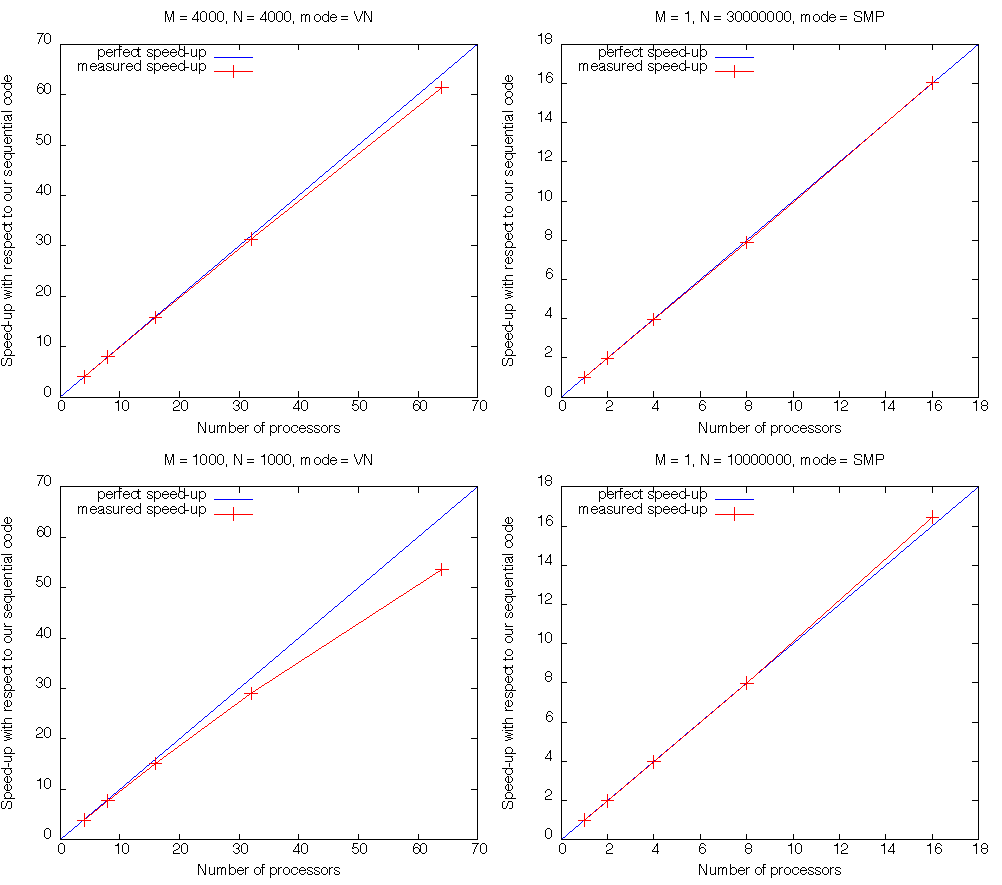
\includegraphics{./speedup-processes-1.pdf}
  \caption{Dependency of speed-up with respect to our sequential implementation, as a function of the number of processes. The perfect (desired) dependency is drawn as a straight line.}
  \label{plot:speedup-processes-1}
\end{figure}

\subsection*{Communication costs}

To resolve ambiguities, we will call \emph{communication time} the wall-clock time of the reduction as measured by the root process.
Note that all communication in both branches of the hybrid algorithm is implemented in terms of a reduction, where the root process is the final destination.

For non-degenerate case there is one communication round preceded by a significant amount of computation.
In this case, the total cost contributed by communication is less than $0.4 \%$ of total running time, that is a completely negligible value.
In fact, total time spent on communication lies within $1$-sigma\footnote{Running times were measured five times for each setting, for the purpose of probabilistic verification of hypotheses we threat them as random variables and apply the framework known from random error analysis in physics.} from $\SI{0}{s}$ therefore we can safely say that it does not contribute to the total running time in any measurable way.

For degenerate case we have to be very careful not to select too many processors for given input size, the following discussion assumes $M = 3 \cdot 10^{7}, N = 1$.
For $P \geq 32$ we have observed spikes in the communication time, which can differ up to three orders of magnitude between different runs on the same input data.
For $P \leq 16$ the communication time per round varies from less than $\SI{40}{\micro s}$ up to almost $\SI{95}{\milli s}$ in rather non-deterministic fashion, i.e. the difference of such magnitude can be observed between different runs on the same input and with the same configuration.
As an example, consider the case of $P = 16$ and DUAL mode in table (\ref{table:communication-cost}), where for five different runs we have obtained results that differ in three orders of magnitude.

\begin{table}[h]
\centering
\begin{tabular}{c|c|c|c|c|c|}
16, VN   & 0.00836 & 0.00190 & 0.00377 & 0.00401 & 0.09402 \\
\hline
16, DUAL & 0.00004 & 0.00004 & 0.00355 & 0.03769 & 0.00004 \\
\hline
16, SMP  & 0.00634 & 0.00004 & 0.00328 & 0.00390 & 0.00106 \\
\hline
4,  VN   & 0.00004 & 0.00004 & 0.01334 & 0.00829 & 0.00004 \\
\hline
4,  DUAL & 0.00004 & 0.00004 & 0.00004 & 0.00041 & 0.00104 \\
\hline
4,  SMP  & 0.00004 & 0.00269 & 0.00876 & 0.01110 & 0.00716 \\
\hline
\end{tabular}
\caption{Total communication time in wall-clock seconds of the root process for $M = 3 \cdot 10^{7}, N = 1$, results from five different runs in each setup. Description column contains the number of processors and operation mode. \label{table:communication-cost}}
\end{table}

We have observed that time spent on each communication round does depend on the time of preceding computation, the dependence is hard to characterise accurately due to very high variance of results\footnote{That is $3$-sigma test fails to separate the value from $\SI{0}{s}$.}, however we can safely say that it is an increasing function of time of the computation.
The reason for this is pretty simple, each communication round is implemented as a reduction, therefore process that is waiting for results has to wait until all other processes synchronise.
The longer preceding computation takes, the bigger differences between execution times of different processes become.
As a consequence, communication time we are measuring includes the time that one process needs to wait for the other until it finishes its job, and this time increases with increasing length of the computation.

\section*{Discussion of the results and final remarks}

We have presented an algorithm, which achieves perfect parallelization in terms of the number of processors for all inputs due to hybrid design.

The algorithm for degenerate case is interesting, because it does not require every processor to know entire input.
If the input size was not limited by the size of the memory of a single processor, we would use this algorithm for all inputs to achieve perfect scalability with respect to memory requirements.

%\newpage

\FloatBarrier
\begin{thebibliography}{9}
    \bibitem{Pearls} J. Bentley \\
        \newblock ,,Programming Pearls - Algorithm Design Techniques''
    \bibitem{TakaokaMSA} T. Takaoka \\
        \newblock ,,Efficient algorithms for the Maximum Subarray Problem by Distance Matrix Multiplication''
    \bibitem{TakaokaHashim} T. Takaoka, M. Hashim \\
        \newblock ,,A Simpler Algorithm for the All Pairs Shortest Path Problem with $O(n^2 \log{n})$ Expected Time''
    \bibitem{MoffatTakaoka} K. Mehlhorn, V. Priebe \\
        \newblock ,,On the All-Pairs Shortest-Path Algorithm of Moffat and Takaoka''
\end{thebibliography}

\newpage
\section*{Appendix A}

The following tables present detailed results of our experiments and speed-up calculations with respect to both our sequential and reference results.

\begin{table}[ht]
\centering
\begin{tabular}{c|c|c|c|c|c|c|c|c|c|}
\hline
$M$ & 250 & 250 & 250 & 1000 & 1000 & 1000 & 4000 & 4000 & 4000 \\
\hline
$N$ & 250 & 1000 & 4000 & 250 & 1000 & 4000 & 250 & 1000 & 4000 \\
\hline
 & 0.004705 & 0.01487 & 0.05884 & 0.01465 & 0.1729 & 0.7014 & 0.05993 & 0.7083 & 10.35 \\
 & 0.004598 & 0.01465 & 0.05795 & 0.01456 & 0.1711 & 0.7007 & 0.05913 & 0.7044 & 10.33 \\
64 & 32.31 & 39.57 & 43.14 & 39.98 & 53.61 & 56.65 & 42.36 & 56.4 & 61.38 \\
 & (105.83) & (201.15) & (275.4) & (313.12) & (219.56) & (308.94) & (549.04) & (542.92) & (269.78) \\
 & 0.00456 & 0.01448 & 0.05762 & 0.01448 & 0.1702 & 0.6991 & 0.05841 & 0.7014 & 10.32 \\
\hline
 & 0.006968 & 0.02371 & 0.0966 & 0.02387 & 0.318 & 1.325 & 0.0983 & 1.331 & 20.27 \\
 & 0.006887 & 0.02361 & 0.09648 & 0.02373 & 0.3158 & 1.321 & 0.09794 & 1.327 & 20.24 \\
32 & 21.57 & 24.56 & 25.91 & 24.53 & 29.05 & 30.05 & 25.57 & 29.94 & 31.33 \\
 & (70.66) & (124.81) & (165.42) & (192.12) & (118.96) & (163.87) & (331.47) & (288.19) & (137.69) \\
 & 0.006815 & 0.02355 & 0.09636 & 0.02366 & 0.3141 & 1.319 & 0.09706 & 1.321 & 20.22 \\
\hline
 & 0.01171 & 0.04201 & 0.1743 & 0.04228 & 0.6104 & 2.564 & 0.1762 & 2.567 & 40.13 \\
 & 0.01148 & 0.0419 & 0.1741 & 0.04195 & 0.6059 & 2.56 & 0.1753 & 2.564 & 40.06 \\
16 & 12.94 & 13.84 & 14.36 & 13.88 & 15.14 & 15.51 & 14.29 & 15.5 & 15.83 \\
 & (42.39) & (70.33) & (91.67) & (108.68) & (62) & (84.56) & (185.19) & (149.15) & (69.57) \\
 & 0.01134 & 0.04178 & 0.1739 & 0.04184 & 0.6024 & 2.554 & 0.1747 & 2.556 & 40.02 \\
\hline
 & 0.02126 & 0.07837 & 0.3297 & 0.07902 & 1.196 & 5.042 & 0.3313 & 5.052 & 79.84 \\
 & 0.02081 & 0.07806 & 0.3291 & 0.07838 & 1.187 & 5.037 & 0.33 & 5.043 & 79.7 \\
8 & 7.14 & 7.43 & 7.6 & 7.43 & 7.73 & 7.88 & 7.59 & 7.88 & 7.96 \\
 & (23.38) & (37.75) & (48.49) & (58.17) & (31.65) & (42.98) & (98.38) & (75.83) & (34.97) \\
 & 0.02059 & 0.07776 & 0.3287 & 0.07795 & 1.18 & 5.028 & 0.3291 & 5.033 & 79.64 \\
\hline
 & 0.04023 & 0.1508 & 0.6405 & 0.1521 & 2.355 & 10 & 0.6426 & 10.02 & 159.3 \\
 & 0.03931 & 0.1502 & 0.6394 & 0.1508 & 2.336 & 9.995 & 0.6406 & 10.01 & 159 \\
4 & 3.78 & 3.86 & 3.91 & 3.86 & 3.93 & 3.97 & 3.91 & 3.97 & 3.99 \\
 & (12.38) & (19.62) & (24.96) & (30.23) & (16.08) & (21.66) & (50.68) & (38.2) & (17.53) \\
 & 0.03884 & 0.1494 & 0.6386 & 0.1501 & 2.322 & 9.978 & 0.639 & 9.984 & 158.9 \\
\hline
\end{tabular}
\caption{Dependence of: maximum and average running times, speedup with respect to our sequential results and reference results (in parentheses) and minimum running times; on the number of processes and input size. Mode of operation is VN.}
\end{table}

\begin{table}[ht]
\centering
\begin{tabular}{c|c|c|c|c|c|c|}
\hline
$M$ & 1 & 1 & 1 & 10000000 & 20000000 & 30000000 \\
\hline
$N$ & 10000000 & 20000000 & 30000000 & 1 & 1 & 1 \\
\hline
 & 0.03178 & 0.06987 & 0.09543 & 0.7247 & 1.543 & 2.052 \\
 & 0.02092 & 0.06129 & 0.06623 & 0.4582 & 0.9762 & 1.069 \\
64 & 45.27 & 31.18 & 43.62 & 2.07 & 1.96 & 2.7 \\
 & 0.01651 & 0.04428 & 0.05112 & 0.2286 & 0.06112 & 0.5998 \\
\hline
 & 0.03525 & 0.07446 & 0.1108 & 0.577 & 1.453 & 1.734 \\
 & 0.03235 & 0.06888 & 0.105 & 0.3407 & 0.9955 & 1.22 \\
32 & 29.28 & 27.75 & 27.51 & 2.78 & 1.92 & 2.37 \\
 & 0.03127 & 0.06553 & 0.1014 & 0.03903 & 0.4486 & 0.6897 \\
\hline
 & 0.06565 & 0.1536 & 0.201 & 0.3542 & 0.208 & 0.2787 \\
 & 0.06341 & 0.1392 & 0.1913 & 0.1352 & 0.1827 & 0.204 \\
16 & 14.94 & 13.73 & 15.1 & 7 & 10.46 & 14.16 \\
 & 0.06017 & 0.1287 & 0.1844 & 0.05898 & 0.1245 & 0.1835 \\
\hline
 & 0.1212 & 0.2481 & 0.3753 & 0.513 & 0.2684 & 1.605 \\
 & 0.1206 & 0.2454 & 0.3713 & 0.2819 & 0.2574 & 0.6429 \\
8 & 7.85 & 7.79 & 7.78 & 3.36 & 7.43 & 4.49 \\
 & 0.12 & 0.2406 & 0.3649 & 0.1199 & 0.2405 & 0.3704 \\
\hline
 & 0.2422 & 0.4903 & 0.7533 & 0.2419 & 0.4904 & 0.7423 \\
 & 0.2401 & 0.4859 & 0.7391 & 0.2397 & 0.4853 & 0.7336 \\
4 & 3.94 & 3.93 & 3.91 & 3.95 & 3.94 & 3.94 \\
 & 0.238 & 0.4806 & 0.7317 & 0.2379 & 0.4794 & 0.7268 \\
\hline
\end{tabular}
\caption{Dependence of: maximum and average running times, speedup with respect to our sequential results and minimum running times; on the number of processes and input size. Mode of operation is VN. We have no reference results for degenerate case.}
\end{table}

\begin{table}[ht]
\centering
\begin{tabular}{c|c|c|c|c|c|c|c|c|c|}
\hline
$M$ & 250 & 250 & 250 & 1000 & 1000 & 1000 & 4000 & 4000 & 4000 \\
\hline
$N$ & 250 & 1000 & 4000 & 250 & 1000 & 4000 & 250 & 1000 & 4000 \\
\hline
 & 0.007019 & 0.02364 & 0.09653 & 0.02381 & 0.3177 & 1.319 & 0.09699 & 1.321 & 20.26 \\
 & 0.006873 & 0.02361 & 0.09638 & 0.02369 & 0.3154 & 1.318 & 0.09684 & 1.319 & 20.23 \\
32 & 21.62 & 24.56 & 25.94 & 24.57 & 29.08 & 30.12 & 25.86 & 30.12 & 31.34 \\
 & (70.8) & (124.81) & (165.59) & (192.44) & (119.11) & (164.25) & (335.24) & (289.94) & (137.76) \\
 & 0.006817 & 0.02354 & 0.09629 & 0.02362 & 0.3137 & 1.316 & 0.09663 & 1.316 & 20.21 \\
\hline
 & 0.01167 & 0.04195 & 0.1742 & 0.04218 & 0.6094 & 2.559 & 0.1746 & 2.564 & 40.12 \\
 & 0.01146 & 0.04174 & 0.174 & 0.04193 & 0.6049 & 2.557 & 0.1742 & 2.56 & 40.05 \\
16 & 12.97 & 13.89 & 14.37 & 13.88 & 15.16 & 15.52 & 14.38 & 15.52 & 15.83 \\
 & (42.46) & (70.6) & (91.72) & (108.73) & (62.1) & (84.66) & (186.36) & (149.39) & (69.58) \\
 & 0.01137 & 0.0415 & 0.1737 & 0.0418 & 0.6014 & 2.553 & 0.1737 & 2.554 & 40.01 \\
\hline
 & 0.0213 & 0.07837 & 0.3296 & 0.07903 & 1.194 & 5.039 & 0.3307 & 5.047 & 79.83 \\
 & 0.02084 & 0.07807 & 0.329 & 0.07838 & 1.184 & 5.035 & 0.3296 & 5.04 & 79.69 \\
8 & 7.13 & 7.43 & 7.6 & 7.43 & 7.75 & 7.88 & 7.6 & 7.88 & 7.96 \\
 & (23.35) & (37.75) & (48.51) & (58.17) & (31.73) & (42.99) & (98.5) & (75.88) & (34.97) \\
 & 0.02061 & 0.07766 & 0.3286 & 0.07797 & 1.178 & 5.027 & 0.3288 & 5.028 & 79.62 \\
\hline
 & 0.04018 & 0.1508 & 0.6403 & 0.1521 & 2.351 & 10 & 0.6424 & 10.02 & 159.3 \\
 & 0.0393 & 0.1502 & 0.6393 & 0.1508 & 2.333 & 9.993 & 0.6404 & 10 & 159 \\
4 & 3.78 & 3.86 & 3.91 & 3.86 & 3.93 & 3.97 & 3.91 & 3.97 & 3.99 \\
 & (12.38) & (19.62) & (24.96) & (30.23) & (16.1) & (21.66) & (50.69) & (38.24) & (17.53) \\
 & 0.03883 & 0.1494 & 0.6384 & 0.1501 & 2.319 & 9.976 & 0.6389 & 9.979 & 158.9 \\
\hline
 & 0.0782 & 0.2955 & 1.262 & 0.2981 & 4.665 & 19.92 & 1.266 & 19.95 & 318.1 \\
 & 0.07633 & 0.2944 & 1.26 & 0.2956 & 4.629 & 19.91 & 1.262 & 19.92 & 317.5 \\
2 & 1.95 & 1.97 & 1.98 & 1.97 & 1.98 & 1.99 & 1.98 & 1.99 & 2 \\
 & (6.38) & (10.01) & (12.67) & (15.42) & (8.12) & (10.87) & (25.72) & (19.2) & (8.78) \\
 & 0.07548 & 0.2928 & 1.258 & 0.2941 & 4.601 & 19.87 & 1.259 & 19.88 & 317.3 \\
\hline
\end{tabular}
\caption{Dependence of: maximum and average running times, speedup with respect to our sequential results and reference results (in parentheses) and minimum running times; on the number of processes and input size. Mode of operation is DUAL.}
\end{table}

\begin{table}[ht]
\centering
\begin{tabular}{c|c|c|c|c|c|c|}
\hline
$M$ & 1 & 1 & 1 & 10000000 & 20000000 & 30000000 \\
\hline
$N$ & 10000000 & 20000000 & 30000000 & 1 & 1 & 1 \\
\hline
 & 0.03 & 0.08194 & 0.09216 & 0.04004 & 0.08278 & 0.1266 \\
 & 0.02915 & 0.06796 & 0.09096 & 0.03253 & 0.07268 & 0.1118 \\
32 & 32.49 & 28.12 & 31.76 & 29.11 & 26.3 & 25.84 \\
 & 0.02875 & 0.05885 & 0.08941 & 0.02894 & 0.05884 & 0.08999 \\
\hline
 & 0.06078 & 0.14 & 0.2154 & 0.05908 & 0.1422 & 0.2159 \\
 & 0.05881 & 0.1234 & 0.1873 & 0.05857 & 0.124 & 0.1882 \\
16 & 16.1 & 15.49 & 15.42 & 16.17 & 15.41 & 15.35 \\
 & 0.05722 & 0.1176 & 0.178 & 0.05776 & 0.1172 & 0.1776 \\
\hline
 & 0.1194 & 0.2417 & 0.3665 & 0.1197 & 0.2417 & 0.3684 \\
 & 0.1182 & 0.2389 & 0.3637 & 0.1184 & 0.2384 & 0.3637 \\
8 & 8.01 & 8 & 7.94 & 8 & 8.02 & 7.94 \\
 & 0.1162 & 0.2351 & 0.3603 & 0.116 & 0.2349 & 0.3603 \\
\hline
 & 0.2395 & 0.4861 & 0.7343 & 0.2396 & 0.4868 & 0.7343 \\
 & 0.2381 & 0.4814 & 0.7277 & 0.2369 & 0.4816 & 0.7255 \\
4 & 3.98 & 3.97 & 3.97 & 4 & 3.97 & 3.98 \\
 & 0.2359 & 0.4736 & 0.7245 & 0.2343 & 0.4737 & 0.715 \\
\hline
 & 0.4816 & 0.9677 & 1.469 & 0.4812 & 0.9676 & 1.469 \\
 & 0.4766 & 0.9563 & 1.455 & 0.4766 & 0.9561 & 1.455 \\
2 & 1.99 & 2 & 1.99 & 1.99 & 2 & 1.99 \\
 & 0.4686 & 0.935 & 1.437 & 0.4687 & 0.9349 & 1.436 \\
\hline
\end{tabular}
\caption{Dependence of: maximum and average running times, speedup with respect to our sequential results and minimum running times; on the number of processes and input size. Mode of operation is DUAL. We have no reference results for degenerate case.}
\end{table}

\begin{table}[ht]
\centering
\begin{tabular}{c|c|c|c|c|c|c|c|c|c|}
\hline
$M$ & 250 & 250 & 250 & 1000 & 1000 & 1000 & 4000 & 4000 & 4000 \\
\hline
$N$ & 250 & 1000 & 4000 & 250 & 1000 & 4000 & 250 & 1000 & 4000 \\
\hline
 & 0.01181 & 0.04193 & 0.1742 & 0.04223 & 0.6093 & 2.559 & 0.1746 & 2.563 & 40.11 \\
 & 0.01149 & 0.04177 & 0.1739 & 0.0419 & 0.6047 & 2.557 & 0.1742 & 2.559 & 40.05 \\
16 & 12.93 & 13.88 & 14.37 & 13.89 & 15.17 & 15.52 & 14.38 & 15.53 & 15.83 \\
 & (42.35) & (70.55) & (91.77) & (108.81) & (62.12) & (84.66) & (186.36) & (149.45) & (69.58) \\
 & 0.01135 & 0.04163 & 0.1737 & 0.04169 & 0.6012 & 2.552 & 0.1738 & 2.553 & 40.01 \\
\hline
 & 0.02129 & 0.07836 & 0.3296 & 0.07909 & 1.193 & 5.039 & 0.3306 & 5.046 & 79.83 \\
 & 0.02081 & 0.07805 & 0.329 & 0.0784 & 1.184 & 5.034 & 0.3296 & 5.039 & 79.69 \\
8 & 7.14 & 7.43 & 7.6 & 7.43 & 7.75 & 7.89 & 7.6 & 7.88 & 7.96 \\
 & (23.38) & (37.76) & (48.51) & (58.15) & (31.73) & (43) & (98.5) & (75.89) & (34.97) \\
 & 0.02054 & 0.0777 & 0.3286 & 0.07801 & 1.177 & 5.026 & 0.3288 & 5.028 & 79.63 \\
\hline
 & 0.04031 & 0.1508 & 0.6402 & 0.1521 & 2.349 & 9.998 & 0.6423 & 10.01 & 159.3 \\
 & 0.03936 & 0.1502 & 0.6392 & 0.1508 & 2.331 & 9.99 & 0.6404 & 9.999 & 159 \\
4 & 3.77 & 3.86 & 3.91 & 3.86 & 3.94 & 3.97 & 3.91 & 3.97 & 3.99 \\
 & (12.36) & (19.62) & (24.97) & (30.23) & (16.12) & (21.67) & (50.69) & (38.25) & (17.53) \\
 & 0.03892 & 0.1494 & 0.6383 & 0.1501 & 2.317 & 9.972 & 0.6387 & 9.976 & 158.9 \\
\hline
 & 0.07815 & 0.2955 & 1.261 & 0.2982 & 4.661 & 19.92 & 1.266 & 19.95 & 318.1 \\
 & 0.07634 & 0.2944 & 1.259 & 0.2956 & 4.625 & 19.9 & 1.262 & 19.92 & 317.5 \\
2 & 1.95 & 1.97 & 1.99 & 1.97 & 1.98 & 1.99 & 1.98 & 1.99 & 2 \\
 & (6.37) & (10.01) & (12.68) & (15.42) & (8.12) & (10.88) & (25.72) & (19.2) & (8.78) \\
 & 0.07544 & 0.2928 & 1.258 & 0.2941 & 4.598 & 19.87 & 1.259 & 19.88 & 317.3 \\
\hline
 & 0.1523 & 0.582 & 2.504 & 0.5872 & 9.245 & 39.73 & 2.512 & 39.79 & 635.1 \\
 & 0.1486 & 0.5798 & 2.5 & 0.5822 & 9.173 & 39.7 & 2.505 & 39.73 & 634 \\
1 & 1 & 1 & 1 & 1 & 1 & 1 & 1 & 1 & 1 \\
 & (3.27) & (5.08) & (6.38) & (7.83) & (4.1) & (5.45) & (12.96) & (9.63) & (4.4) \\
 & 0.1469 & 0.5767 & 2.496 & 0.5793 & 9.119 & 39.63 & 2.498 & 39.64 & 633.5 \\
\hline
\end{tabular}
\caption{Dependence of: maximum and average running times, speedup with respect to our sequential results and reference results (in parentheses) and minimum running times; on the number of processes and input size. Mode of operation is SMP.}
\end{table}

\begin{table}[ht]
\centering
\begin{tabular}{c|c|c|c|c|c|c|}
\hline
$M$ & 1 & 1 & 1 & 10000000 & 20000000 & 30000000 \\
\hline
$N$ & 10000000 & 20000000 & 30000000 & 1 & 1 & 1 \\
\hline
 & 0.05818 & 0.1195 & 0.1812 & 0.05814 & 0.1194 & 0.1812 \\
 & 0.05758 & 0.1185 & 0.1802 & 0.05758 & 0.1185 & 0.1802 \\
16 & 16.45 & 16.13 & 16.03 & 16.45 & 16.13 & 16.03 \\
 & 0.05717 & 0.1178 & 0.1796 & 0.05717 & 0.1179 & 0.1797 \\
\hline
 & 0.1201 & 0.2422 & 0.369 & 0.1202 & 0.2422 & 0.3691 \\
 & 0.1185 & 0.2409 & 0.366 & 0.1185 & 0.2408 & 0.366 \\
8 & 7.99 & 7.93 & 7.89 & 7.99 & 7.94 & 7.89 \\
 & 0.1177 & 0.2398 & 0.3617 & 0.1177 & 0.2398 & 0.3617 \\
\hline
 & 0.24 & 0.4902 & 0.7317 & 0.24 & 0.4902 & 0.7316 \\
 & 0.2379 & 0.4809 & 0.7272 & 0.2379 & 0.4809 & 0.7271 \\
4 & 3.98 & 3.97 & 3.97 & 3.98 & 3.97 & 3.97 \\
 & 0.2366 & 0.4717 & 0.7192 & 0.2367 & 0.4716 & 0.7193 \\
\hline
 & 0.4855 & 0.9725 & 1.476 & 0.4855 & 0.9725 & 1.476 \\
 & 0.4783 & 0.9576 & 1.458 & 0.4783 & 0.9576 & 1.458 \\
2 & 1.98 & 2 & 1.98 & 1.98 & 2 & 1.98 \\
 & 0.4666 & 0.9355 & 1.446 & 0.4666 & 0.9355 & 1.446 \\
\hline
 & 0.9625 & 1.943 & 2.955 & 0.9625 & 1.943 & 2.956 \\
 & 0.9471 & 1.911 & 2.889 & 0.9471 & 1.911 & 2.889 \\
1 & 1 & 1 & 1 & 1 & 1 & 1 \\
 & 0.9241 & 1.861 & 2.822 & 0.9241 & 1.861 & 2.822 \\
\hline
\end{tabular}
\caption{Dependence of: maximum and average running times, speedup with respect to our sequential results and minimum running times; on the number of processes and input size. Mode of operation is SMP. We have no reference results for degenerate case.}
\end{table}

%%%%%%%%%%%%%%%%%%%%%%%%%%%%%%%%%%%%%%%%%%%%%%%%%%%%%%%%%%%%%%%%%%%%%%%%%%%%%%%%%%%%%%%%%%%%%%%%%%%%
\end{document}
% vim: noet:sw=2:ts=2:tw=160:wrap
